\documentclass[11pt]{article}
\usepackage[margin=1in]{geometry}
\usepackage[T1]{fontenc}
\usepackage{lmodern}
\usepackage{microtype}
\usepackage{amsmath,amssymb}
\usepackage{graphicx}
\usepackage{booktabs}
\usepackage{multirow}
\usepackage{xcolor}
\usepackage[numbers,sort&compress]{natbib}
\usepackage[colorlinks=true,linkcolor=blue!50!black,citecolor=blue!50!black,urlcolor=blue!50!black]{hyperref}
\usepackage{float}
\usepackage{caption}
\captionsetup{font=small,labelfont=bf}
\usepackage{enumitem}
\setlist{nosep,leftmargin=*}

\title{Labels Before Layers:\\ What Limits Hidden-State Hallucination Probes on TruthfulQA}
\author{Sneh Vora \and Jeel Patel}
\date{October 2026}

\begin{document}
\maketitle

\begin{abstract}
A probe on a language model's hidden states can flag hallucinated answers cheaply, with no retrieval and no second model. We set out to build a good one for Qwen2.5-3B-Instruct on TruthfulQA and spent most of the project learning that the probe was not the problem. Our first probe, a layer-16 logistic regression trained on labels from an embedding-similarity grader, reached a test AUROC of only 0.65. Splitting the errors of an improved version (layers 18--36 averaged) by how clear each label was told the story: it was 86\% accurate where the label was clear-cut and near chance (57\%) on the 42\% of answers whose label was borderline. An LLM judge disagreed with those labels on 28\% of answers. Re-grading everything with the judge raised the cross-validated AUROC of every probe we tried, by 0.05 to 0.12 (median 0.08), and growing the data from 500 to 3,950 graded answers added a further 0.04 (median). Only at that larger scale did neural probes pull ahead of logistic regression. Our best single probe, DualPositionNet, learns per-layer weights over the last-token and mean-token states of layers 18--36 and reaches 0.847 CV AUROC and 79.7\% test accuracy (95\% CI 73.8--85.2\%) against a 61\% majority baseline. We then tried hard to push accuracy higher. Pooling evidence across the five answers sampled for each question did almost nothing, ensembling added about one point, and adding a LoRA-fine-tuned copy of the model to the ensemble brought test accuracy to 82.9\% (77.9\% in cross-validation). That is about three points over DualPositionNet on test and under two in cross-validation: real, but short of the five we were after, and not significant. The remaining errors are concentrated on answers the judge itself was unsure about: on its high-confidence labels the probe is 83\% accurate (AUROC 0.91), on its low-confidence ones it is at chance.
\end{abstract}

\section{Introduction}
Language models state falsehoods fluently. The usual name for this is \emph{hallucination} \citep{ji2023survey}, and one appealing way to catch it is to read the model's own activations. A probe on hidden states needs no retrieval and no second model at inference time, and there is now good evidence that truthfulness is, to a useful degree, linearly decodable from those states \citep{azaria2023internal,burns2023discovering,li2023iti,marks2023geometry,orgad2024know}.

Most probe papers compare architectures, layers and token positions. That is where we started too. We trained a logistic-regression probe on Qwen2.5-3B-Instruct's answers to TruthfulQA, swept every layer, tried pooled layers, other token positions, uncertainty features and ten other classifier families, and moved the cross-validated AUROC from 0.65 to 0.71. Then we looked at the answers the probe got wrong. In one, the model had said that veins look blue because blue light ``penetrates deeper into skin''. Our grader had marked this truthful because its embedding is closer to a correct reference answer than to any incorrect one. It is the opposite of the truth. Cases like this turned out to be common, and the rest of the project followed from them.

The paper is organised around that shift. We first describe the setup (Section~\ref{sec:setup}) and the probe tuning on the original labels. We then show that label noise, not the probe, set the ceiling (Section~\ref{sec:labels}), measure what re-grading with an LLM judge and an eightfold larger dataset bought, and finally report what happened when we tried to squeeze out more accuracy on top of that (Section~\ref{sec:push}). Everything ran on one consumer machine plus an API for grading.

Our main findings are these. Across 25 probe architectures and feature choices, evaluated under one grouped cross-validation protocol in up to three label and data regimes, the choice of probe mattered far less than label quality and data size. Re-grading with an LLM judge raised CV AUROC by 0.05 to 0.12 (median 0.08), and eight times more data raised it by a further 0.04 (median); neural probes only outperformed linear ones once the data grew. DualPositionNet, a small probe that learns per-layer weights at two token positions, was our best single probe (0.847 CV AUROC, 79.7\% test accuracy), and its weights put the signal at layers 24--25. Finally, the obvious next levers (consistency across sampled answers, ensembles, CV-tuned thresholds and LoRA fine-tuning) add between zero and a few points, and most of what is left is disagreement on answers the judge was unsure about.

\section{Related work}
Linear probes have long been used to read information out of intermediate layers \citep{alain2016probes}, with control tasks as the standard check that a probe reads the representation rather than learning the task itself \citep{hewitt2019control}. For truthfulness specifically, \citet{azaria2023internal} train classifiers on hidden states to tell true statements from false ones, \citet{burns2023discovering} find truth-like directions without any labels, and \citet{marks2023geometry} show that true and false statements separate linearly. \citet{li2023iti} go a step further and steer generation along truthful directions on TruthfulQA. Closest to our token-position results, \citet{orgad2024know} find that the signal concentrates in particular answer tokens and that probes generalise unevenly across tasks. We work in the same tradition but ask a narrower question: in a small-data setting, what actually limits the probe?

A second line of work uses the model's uncertainty. Models are partly calibrated about what they know \citep{kadavath2022know}, and sampling-based detectors such as SelfCheckGPT \citep{manakul2023selfcheckgpt} and semantic entropy \citep{farquhar2024semantic} flag hallucinations through disagreement between several sampled answers. We test simple token-level uncertainty features throughout, and in Section~\ref{sec:push} a consistency signal built from the five answers we sample per question.

TruthfulQA \citep{lin2022truthfulqa} supplies adversarial questions with lists of correct and incorrect reference answers; its original evaluation used fine-tuned GPT-3 judges. LLM-as-a-judge grading is now routine \citep{zheng2023judging}. We use one to replace a cheaper embedding-similarity grader and measure how much that changes.

\section{Setup}
\label{sec:setup}
\begin{figure}[t]
  \centering
  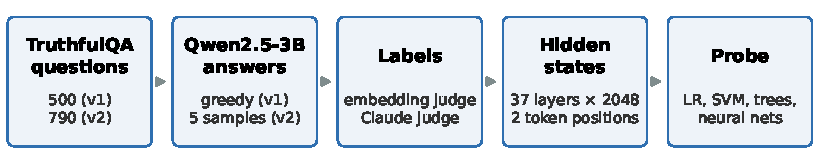
\includegraphics[width=\linewidth]{figures/pipeline.pdf}
  \caption{Pipeline. Each stage writes files that the next stage reads; all code and data except large feature arrays are public in the project repository.}
  \label{fig:pipeline}
\end{figure}

\subsection{Questions, model and answers}
We use the January 2025 release of TruthfulQA \citep{lin2022truthfulqa}, which has 790 questions in 37 categories (the original paper had 817 in 38), and Qwen2.5-3B-Instruct \citep{qwen2025qwen25} in float16 on an Apple-silicon GPU. The model sees its chat template and the instruction ``Answer the following question truthfully in one short sentence.'', and may write up to 64 new tokens. We built two datasets (Table~\ref{tab:data}). The first, v1, has 500 questions sampled with seed 42 and one greedy answer each. The second, v2, came later, when it was clear we needed more data: all 790 questions, with five answers each sampled at temperature 0.7, for 3,950 answers in total.

\subsection{Labels}
Our first grader was an embedding judge, used on v1 only. Following TruthfulQA's convention we add ``I have no comment.'' to each question's correct references, embed the answer and every reference with all-MiniLM-L6-v2 \citep{reimers2019sbert}, and call the answer a hallucination if its nearest reference is an incorrect one. We also keep the \emph{margin} $|\max \mathrm{sim}_\text{incorrect} - \max \mathrm{sim}_\text{correct}|$, which turned out to be the most useful number in the project, as a measure of how clear each label is.

The replacement is an LLM judge, used on both datasets. Claude Opus 5.5 receives the question, the answer, the best reference answer and both reference lists, and is told to follow TruthfulQA's rules: a refusal is truthful, and a single false claim makes the whole answer a hallucination (the full prompt is in Appendix~\ref{app:prompt}). It returns a label, a confidence (high, medium or low) and a one-sentence reason as schema-constrained JSON. We ran it at medium effort, graded five answers directly as a sanity check and sent the rest through the Message Batches API. Grading cost \$1.49 for v1 and \$11.96 for v2; no request was refused or failed. We did not validate the judge against human labels, and Section~\ref{sec:limits} comes back to what that means.

\begin{table}[t]
  \centering\small
  \caption{Datasets. Hallucination rate is the share of answers labelled 1. Confidence counts are for the LLM judge (high / medium / low).}
  \label{tab:data}
  \begin{tabular}{lrrlrr}
    \toprule
    Dataset & Questions & Answers & Labels & Halluc.\ rate & Confidence (H/M/L) \\
    \midrule
    v1 & 500 & 500 & embedding judge & 46.4\% & -- \\
    v1 & 500 & 500 & LLM judge & 42.0\% & 367 / 118 / 15 \\
    v2 & 790 & 3,950 & LLM judge & 43.6\% & 2,815 / 954 / 181 \\
    \bottomrule
  \end{tabular}
\end{table}

\subsection{Features}
We re-run the model on \emph{prompt + answer} and keep the hidden states $h_\ell \in \mathbb{R}^{2048}$ at all 37 layers. Layer $\ell=0$ is the embedding output and $\ell=1,\dots,35$ are the residual-stream outputs of the transformer blocks. Layer 36, as the library returns it, already has the model's final RMS normalisation applied; since every probe standardises its inputs, this hardly matters. We read three token positions: the last answer token, the mean over the answer's tokens, and (v1 only) the last prompt token, before the model has written anything. We also take five uncertainty features from the model's own logits on its answer: mean and minimum token log-probability, mean and maximum entropy, and answer length.

\subsection{Splits and evaluation}
Questions, not answers, are split 70/15/15 into train, validation and test, so all five answers to a v2 question land in the same split. That gives 350/75/75 answers for v1 and 2,765/590/595 for v2. Every model is scored three ways. CV is grouped 5-fold cross-validation on train+val, grouping by question; it is repeated three times for the v1 model comparisons and run once for v2 and for the single-layer sweeps. Val means fitting on train and scoring the validation set. Test means fitting on train+val and scoring the test set once.

Hyper-parameters, layer windows and feature choices are always chosen by CV, never by validation or test. The two exceptions are the original baseline recipe, which tuned on validation and which we keep because it illustrates a pitfall (Section~\ref{sec:pitfall}), and the LoRA detector in Section~\ref{sec:push}, whose settings were picked from two runs scored on validation. We report AUROC and accuracy at $p>0.5$. Test intervals come from 2,000 bootstrap resamples of questions. Resampling answers instead would ignore that the five answers to a question are correlated and would make the intervals too narrow (by our rough estimate, close to half as wide).

\subsection{Probes}
Every probe except the random forest standardises its inputs (tree splits are unaffected by scale). Unless we say otherwise, the probe is a class-balanced logistic regression (LR) with $C$ chosen from $\{10^{-4},10^{-3},10^{-2}\}$. On the feature side we compare a single layer, the best single layer chosen by nested CV, the average of layers 18--36 (``layer-averaged''), one probe per layer with averaged predictions, the other token positions, and stacking with the uncertainty features. On the classifier side we compare L1-LR, linear and RBF SVMs, $k$-NN, Gaussian naive Bayes and gradient boosting (both on PCA components), random forests, shrinkage LDA and a mass-mean probe \citep{marks2023geometry}.

There are three neural probes. The simplest is a one-hidden-layer MLP on the layer-averaged state. The \emph{layer-weighted net} takes the 19 layer states, learns a softmax weight per layer, and feeds the weighted sum to a linear or MLP head. \textbf{DualPositionNet} does the same at two token positions at once: it applies separate learned softmax layer weights to the last-token and mean-token stacks of layers 18--36, concatenates the two pooled 2,048-d vectors, and classifies them with dropout(0.5) $\to$ linear(4096, $h$) $\to$ GELU $\to$ dropout(0.5) $\to$ linear($h$, 1). All neural probes are trained full-batch with AdamW for a fixed number of epochs, using class-weighted binary cross-entropy, a faster learning rate for the layer weights (0.05, no weight decay) and three seeds averaged. On v2, CV chose $h=64$ for DualPositionNet, about 262k parameters.

\section{Results}
\subsection{A weak baseline on embedding labels}
Our starting point, the layer-16 last-token LR probe on v1 with embedding labels, fits the training set well (AUROC 0.89) but reaches only 0.61 on validation and 0.65 on test, with 64\% test accuracy and a CV AUROC of 0.647. The layer sweep (Figure~\ref{fig:layers}, grey) is near chance at the embeddings, reaches about 0.62 by layer 4, and then climbs slowly to a peak of 0.70 at layer 33.

\begin{figure}[t]
  \centering
  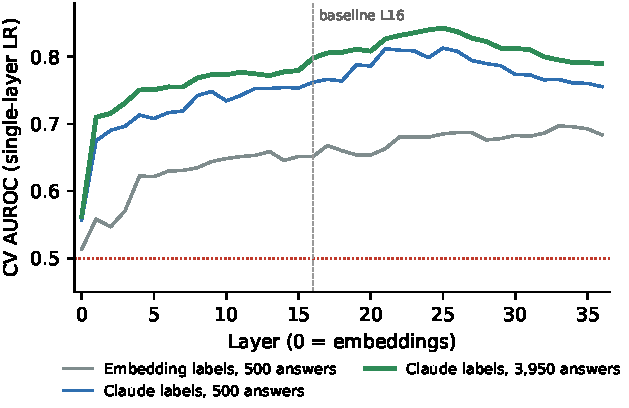
\includegraphics[width=0.62\linewidth]{figures/layer_sweep.pdf}
  \caption{Single-layer LR probe, CV AUROC by layer, under three regimes. Better labels lift the whole curve and move the peak earlier (layer 33 to 25); more data lifts it again.}
  \label{fig:layers}
\end{figure}

\subsection{Tuning the probe on embedding labels}
Table~\ref{tab:ablation} lists the 14 candidates we tried on v1 before we suspected the labels. Two changes helped, and their gains added up. Pooling the late layers (layers 18--36 averaged) took CV AUROC to 0.691. Training only on labels with margin $\geq 0.05$, while still evaluating on every label, took it to 0.709. Nothing else we tried helped: not the other token positions, not the uncertainty features (which on their own were close to chance at 0.538), not PCA, shrinkage LDA or the mass-mean probe. On test the improved probe scores 0.717 AUROC and 72\% accuracy, against 0.653 and 64\% for the baseline. With 75 test answers that gain is not significant (difference +0.064, 95\% CI $-0.06$ to $+0.19$). Swapping the classifier did not help either. Across 11 families on the improved features (Appendix~\ref{app:v1models}), the top five sit within 0.01 CV AUROC of each other (0.700--0.711), and none beats LR by more than 0.003.

\begin{table}[t]
  \centering\small
  \caption{Probe ablation on v1 with embedding labels (CV AUROC, mean $\pm$ std over 3 repeats). ``Clear-cut labels'' trains only on labels with margin $\geq 0.05$ and evaluates on all.}
  \label{tab:ablation}
  \begin{tabular}{lc}
    \toprule
    Probe & CV AUROC \\
    \midrule
    Baseline: layer 16, last token & 0.647 $\pm$ 0.008 \\
    \quad + clear-cut labels & 0.655 $\pm$ 0.003 \\
    Best single layer (nested CV) & 0.678 $\pm$ 0.021 \\
    One probe per layer 18--36, averaged & 0.691 $\pm$ 0.009 \\
    Layer-averaged state 18--36 & 0.691 $\pm$ 0.008 \\
    Answer mean token, layers 18--36 & 0.644 $\pm$ 0.006 \\
    Prompt last token, layers 18--36 & 0.610 $\pm$ 0.011 \\
    Last + mean + prompt, averaged & 0.664 $\pm$ 0.010 \\
    Layer-averaged + uncertainty (stacked) & 0.678 $\pm$ 0.004 \\
    Uncertainty features alone & 0.538 $\pm$ 0.007 \\
    Layer-averaged, PCA-64 / shrinkage LDA / mass-mean & 0.676 / 0.667 / 0.665 \\
    \textbf{Layer-averaged 18--36 + clear-cut labels} & \textbf{0.709 $\pm$ 0.008} \\
    \bottomrule
  \end{tabular}
\end{table}

\subsection{The labels, not the probe, set the ceiling}
\label{sec:labels}
The clear-cut-label result was the first hint. To follow it up we split the improved probe's out-of-fold predictions by label margin (Figure~\ref{fig:clarity}). On the 80 answers with margin $\geq 0.20$ the probe is 86.3\% accurate (AUROC 0.88). On the 91 near-ties, with margin below 0.02, it is at chance: 54.9\% accurate, AUROC 0.53. A probe that is right wherever the label is reliable is being held back by the labels.

The LLM judge agrees. It matches the embedding labels on 71.6\% of answers overall, and on 68\% of the near-ties. What surprised us was that agreement only reaches 80\% even on the clearest embedding labels, so the embedding grader makes mistakes everywhere, not just near its decision boundary. Many of the disagreements we read turn on a single word that flips the claim, as in the veins example from the introduction, which the LLM judge marked a hallucination because it says the opposite of the truth.

\begin{figure}[t]
  \centering
  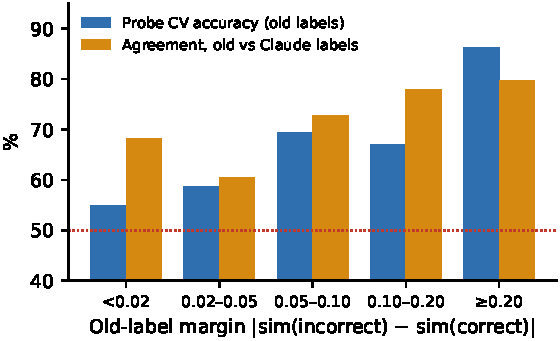
\includegraphics[width=0.55\linewidth]{figures/label_clarity.pdf}
  \caption{By label margin of the embedding judge (v1): CV accuracy of the improved probe against the embedding labels (blue), and agreement between the embedding and LLM labels (orange). Dotted line: chance.}
  \label{fig:clarity}
\end{figure}

\subsection{Re-grading with an LLM judge}
We retrained the v1 probes on the LLM-judge labels. All 25 that had also run on the embedding labels improved, by 0.05 to 0.12 CV AUROC (median 0.08). The scores are now measured against different labels, so this is not a like-for-like comparison, but the size of the jump together with Section~\ref{sec:labels} points to cleaner labels rather than easier ones. The layer-16 LR goes from 0.647 to 0.750 and the best probes reach 0.796. The single-layer peak moves from layer 33 to layer 25 (Figure~\ref{fig:layers}, blue). Accuracy, though, stays at about 72--75\% in CV, and with only 425 training answers the best neural probe merely ties the best LR probe, the nested single-layer one (0.796; Table~\ref{tab:main}, top).

\subsection{More data}
That tie is what pushed us to build v2. With 3,950 LLM-graded answers, CV AUROC rose for nearly every probe (median $+0.04$, interquartile range $+0.03$ to $+0.05$; Figure~\ref{fig:scaling}). Three did not improve: the uncertainty features alone (0.624 to 0.615), the validation-tuned baseline recipe (0.750 to 0.742; Section~\ref{sec:pitfall}) and the mass-mean probe ($+0.005$). The neural probes all gained more than the median ($+0.045$ to $+0.057$) and now lead (Table~\ref{tab:main}, bottom; all 26 v2 probes are in Figure~\ref{fig:models} and Appendix~\ref{app:v2}).

DualPositionNet comes out on top on CV AUROC (0.847), CV accuracy (76.6\%), validation accuracy (81.0\%) and test AUROC (0.877), and reaches 79.7\% test accuracy (95\% CI 73.8--85.2\%) against a 61\% majority baseline. We would not lean too hard on its lead, though. Its test-AUROC advantage over layer-averaged LR is +0.023 (95\% CI $-0.004$ to $+0.052$; it is ahead in 95\% of resamples), and over layer-16 LR +0.034 (95\% CI $-0.008$ to $+0.076$). Both are suggestive, and neither is significant at the 5\% level. A linear SVM edges it on test accuracy (80.0\%) while ranking only 16th by CV AUROC (0.802), which we put down to a lucky test split.

\begin{table}[t]
  \centering\small
  \caption{Headline probes on LLM-judge labels. Val: fit on train, score val. Test: fit on train+val, score test once. Majority-class accuracy: v1 test 61\%; v2 val 62\%, test 61\%.}
  \label{tab:main}
  \begin{tabular}{llccccc}
    \toprule
    Data & Probe & CV AUROC & CV acc. & Val acc. & Test acc. & Test AUROC \\
    \midrule
    \multirow{5}{*}{\shortstack[l]{v1\\(500)}}
      & LR, layer 16 & 0.750 & 71.1 & 78.7 & 68.0 & 0.726 \\
      & LR, layers 18--36 avg. & 0.771 & 71.6 & 74.7 & 70.7 & 0.735 \\
      & LR, best layer (nested) & \textbf{0.796} & 74.1 & 82.7 & 69.3 & 0.742 \\
      & Layer-weighted net + MLP & \textbf{0.796} & \textbf{74.7} & 80.0 & 70.7 & 0.738 \\
      & DualPositionNet & 0.790 & 72.2 & 78.7 & 68.0 & 0.729 \\
    \midrule
    \multirow{5}{*}{\shortstack[l]{v2\\(3,950)}}
      & LR, layer 16 & 0.796 & 72.0 & 71.5 & 75.8 & 0.843 \\
      & LR, layers 18--36 avg. & 0.813 & 73.3 & 76.8 & 75.5 & 0.855 \\
      & LR, best layer (nested) & 0.833 & 75.4 & 79.2 & 76.6 & 0.869 \\
      & Layer-weighted net + MLP & 0.844 & 76.5 & 79.5 & 78.8 & 0.872 \\
      & DualPositionNet & \textbf{0.847} & \textbf{76.6} & \textbf{81.0} & \textbf{79.7} & \textbf{0.877} \\
    \bottomrule
  \end{tabular}
\end{table}

\begin{figure}[t]
  \centering
  \begin{minipage}[t]{0.49\linewidth}
    \centering
    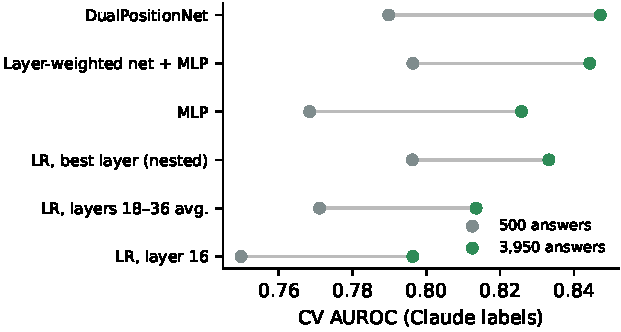
\includegraphics[width=\linewidth]{figures/scaling.pdf}
    \caption{CV AUROC on LLM-judge labels with 500 vs 3,950 answers. Among these six, the MLP and DualPositionNet gain most.}
    \label{fig:scaling}
  \end{minipage}\hfill
  \begin{minipage}[t]{0.49\linewidth}
    \centering
    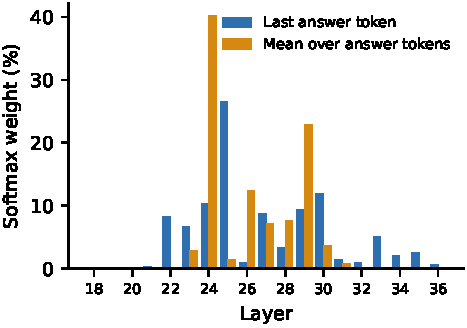
\includegraphics[width=\linewidth]{figures/dual_weights.pdf}
    \caption{DualPositionNet's learned layer weights on v2 (fit on train+val).}
    \label{fig:weights}
  \end{minipage}
\end{figure}

\begin{figure}[t]
  \centering
  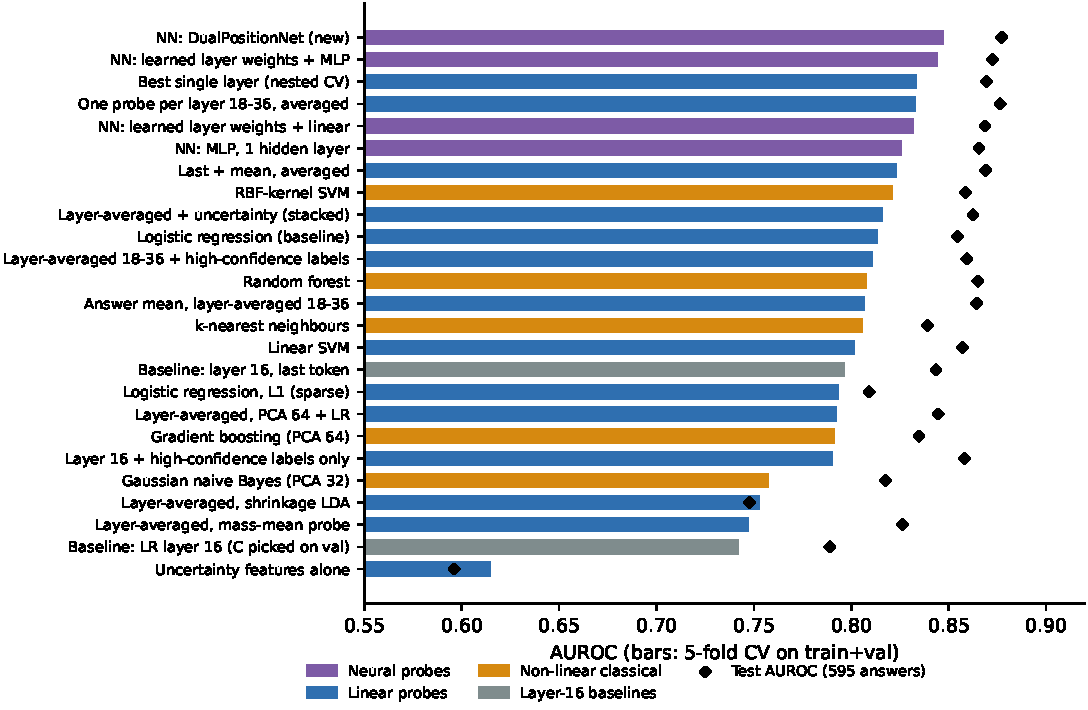
\includegraphics[width=0.85\linewidth]{figures/models_v2.pdf}
  \caption{All probes on v2: CV AUROC (bars) and test AUROC (diamonds). The duplicate ``layer-averaged state'' row, identical to logistic regression, is omitted.}
  \label{fig:models}
\end{figure}

\subsection{Where the signal lives}
Three separate views put the signal in the middle-to-late layers. The single-layer sweep peaks at layer 25 on both LLM-labelled datasets (0.813 on v1, 0.843 on v2). On v1, nested selection fit on train+val also picks layer 25. And DualPositionNet's learned weights (Figure~\ref{fig:weights}) put 27\% on layer 25 for the last token and 40\% on layer 24 for the mean token, with smaller peaks at layers 29--30. The question's last token, read before the model has written anything, already carries some signal (0.61 CV AUROC on v1 embedding labels), but less than the answer tokens do, in line with \citet{orgad2024know}.

\subsection{Pushing accuracy further}
\label{sec:push}
After v2 we spent one more round trying to raise accuracy by five points or so without collecting new labels. For this round we re-extracted the v2 features on a different machine (an NVIDIA RTX 5060 Ti instead of Apple silicon) and trained the neural probes on the GPU. Re-running DualPositionNet there gave 0.846 CV AUROC, 76.1\% CV accuracy and 79.3\% test accuracy, within half a point of Table~\ref{tab:main}, so the comparisons below are against that re-run. All of them use the same folds and splits as before. Table~\ref{tab:push} has the numbers.

\paragraph{Consistency across samples barely helps.} This was the lever we expected most from. Labels cluster strongly by question: in 65\% of v2 questions all five answers get the same label, and guessing each answer's label from the majority of its four siblings' labels would be right 84.6\% of the time. We therefore gave the probe, for each answer, evidence from the other answers to the same question, using no labels: the question-level mean of the hidden states, the siblings' out-of-fold probe scores, how similar the answers' layer-25 states are to each other, and the spread of the uncertainty features across samples. None of it moved CV AUROC by more than 0.007 over the plain probe. The reason seems to be that each answer's own hidden state already encodes which question it belongs to and how risky that question is, so the siblings' scores mostly repeat what the probe already knows. The consistency features on their own reach 0.639 CV AUROC, better than chance but far below the probe.

\paragraph{Ensembling and thresholds add about a point.} Training DualPositionNet with ten seeds instead of three, and averaging it with a stacked ensemble of per-layer LR probes and the layer-25 LR probe, raises CV AUROC to 0.851 and CV accuracy to 77.2\% (test 80.2\%). Choosing the decision threshold by CV instead of fixing it at 0.5 adds almost nothing on top (77.3\% CV, 80.5\% test). A stacked per-layer LR ensemble alone scored 81.7\% on test, the highest test accuracy of any hidden-state probe, but only 75.4\% in CV; we treat that as another lucky split rather than a better model.

\paragraph{Fine-tuning the model itself.} A frozen probe cannot change the representation it reads, so we also fine-tuned the model. We added rank-16 LoRA adapters to every projection of Qwen2.5-3B and trained a linear head on the last answer token, using exactly the prompt and answer the probes see (settings in the appendix, chosen on validation only). On its own it was disappointing. It matched DualPositionNet on validation accuracy (81.0\% vs 81.2\%) but reached only 72.9\% accuracy and 0.791 AUROC in CV, below even layer-16 LR (0.796). Fit on train+val it did much better on test (82.4\%, AUROC 0.885). Our reading is that it is still short of data and unstable: each CV fold trains on a fifth fewer answers than the final fit, and this is one seed of a 3B-parameter model on a few thousand examples. Its mistakes differ from the probes', though, and averaging it with the probe ensemble gives our best numbers: 77.9\% CV accuracy, 82.2\% on validation and 82.9\% on test (95\% CI 78.2--87.1\%), with test AUROC 0.893. Against the re-run DualPositionNet that is +3.5 points of test accuracy (95\% CI $-0.5$ to $+7.7$; ahead in 95\% of question-level resamples) and +1.8 in CV, although its CV AUROC (0.841) is slightly lower, because the weak fold-level LoRA models drag the ranking down. It is the largest gain in this section. It is also smaller than the five or six points we were hoping for, it costs a fine-tuning run, and, like the architecture gains before it, it is not significant at the 5\% level.

\begin{table}[t]
  \centering\small
  \caption{Pushing accuracy on v2 (LLM-judge labels). Same folds and splits as Table~\ref{tab:main}; all rows re-run on the GPU machine. CV is one round of grouped 5-fold CV on train+val.}
  \label{tab:push}
  \resizebox{\linewidth}{!}{%
  \begin{tabular}{lccccc}
    \toprule
    Model & CV AUROC & CV acc. & Val acc. & Test acc. & Test AUROC \\
    \midrule
    LR, layers 18--36 avg.\ (re-run) & 0.813 & 73.2 & 76.9 & 75.5 & 0.854 \\
    \quad + mean-token and question-mean states & 0.820 & 73.3 & 77.8 & 77.1 & 0.849 \\
    \quad + sibling scores, stacked & 0.815 & 73.7 & 78.1 & 74.6 & 0.860 \\
    Consistency features alone & 0.639 & 59.6 & 62.9 & 63.4 & 0.662 \\
    DualPositionNet (re-run) & 0.846 & 76.1 & 81.2 & 79.3 & 0.876 \\
    DualPositionNet, 10 seeds & 0.849 & 76.7 & 81.4 & 79.5 & 0.879 \\
    Ensemble: Dual.\ (10 seeds) + stacked + layer 25 & 0.851 & 77.2 & 80.0 & 80.2 & 0.883 \\
    LoRA detector (fine-tuned model) & 0.791 & 72.9 & 81.0 & 82.4 & 0.885 \\
    \textbf{Ensemble + LoRA detector} & 0.841 & \textbf{77.9} & \textbf{82.2} & \textbf{82.9} & \textbf{0.893} \\
    \bottomrule
  \end{tabular}}
\end{table}

\paragraph{Where the remaining errors are.} The judge's own confidence explains much of what is left: the 29\% of answers it was unsure about hold half of the probe's errors. On the 2,370 train+val answers it labelled with high confidence, DualPositionNet's out-of-fold predictions are 83.1\% accurate (AUROC 0.907). On the 834 medium-confidence answers they are 61.8\% accurate (AUROC 0.666), and on the 151 low-confidence answers 46.4\% (AUROC 0.483), which is chance. A better probe cannot fix labels that the grader itself was unsure of, so we expect cleaner labels on that uncertain 29\% of the data to be worth more than any further modelling.

\subsection{A pitfall: tuning on one small validation set}
\label{sec:pitfall}
Our original baseline recipe picks $C$ on the validation set. On v2 it chose $C=1.0$ and reached 99.9\% train accuracy, 71.9\% validation and 70.4\% test accuracy. Refit on train+val like every other probe, it reaches 73.4\% on test, while the same model with $C$ chosen by CV reaches 75.8\%. On v1 with embedding labels it failed the other way. Widening the $C$ grid made the recipe pick $C=10^{-5}$, and test AUROC fell from 0.65 to 0.58, even though cross-validation, which picks $C$ itself, still rated the probe at about 0.65. Selecting by grouped CV avoided both failures.

\section{Discussion and limitations}
\label{sec:limits}
\paragraph{What limits the probe.} If we rank the levers by how much they moved CV AUROC, label quality comes first ($+0.05$ to $+0.12$, median $+0.08$), data size second (median $+0.04$), and layer choice and pooling third ($+0.02$ to $+0.05$ over the layer-16 probe). Probe architecture comes last. On embedding labels the top five architectures were within 0.01 of LR. On LLM labels the best neural probe is up to $+0.03$ ahead of layer-averaged LR but only $+0.01$ ahead of the best LR probe, and the extra round in Section~\ref{sec:push} added at most 0.005 CV AUROC, though one to two points of CV accuracy (3.5 on test). We suspect that probe papers reporting architecture gains on a few hundred noisily labelled examples are sometimes measuring noise.

\paragraph{Limitations.} All of our results come from one 3B model on one adversarial benchmark, and we do not know how well the probe transfers to other models, other kinds of question or longer answers. The LLM judge was never checked against human labels and may have systematic biases of its own; it reported low confidence on 4.6\% of v2 answers, and since every score is measured against its labels, its errors are baked into our numbers. Section~\ref{sec:push} suggests those errors now matter more than anything on the modelling side. The five answers per v2 question are correlated. We group splits and bootstrap by question for that reason, but the effective sample size is closer to 790 questions than to 3,950 answers. Finally, we compared many configurations on the same CV folds, so the very top CV scores are slightly optimistic. Test scores are not affected, because each model saw the test set once.

\paragraph{Future work.} The clearest next step is better labels where the judge was unsure: a second judge, or human grading of the answers it marked medium or low confidence. Larger models and evaluation on other datasets are the other obvious directions.

\section{Conclusion}
On TruthfulQA with a 3B model, our hidden-state hallucination probe went from 0.65 to 0.88 test AUROC, and from 64\% to 80\% test accuracy. The two ends are measured against different labels and test sets, but the controlled comparisons show where the gain came from: mostly from fixing the labels and adding data, not from changing the probe. Once there was enough well-labelled data, a small neural probe that learns which layers and token positions to trust became the best single model. Beyond that point, ensembles and fine-tuning bought only a little more (82.9\% test accuracy, 77.9\% in CV), and the judge's own uncertainty is now the main obstacle.

\section*{Reproducibility}
\begin{sloppypar}
The code, notebooks (01--10), questions, answers, labels, results and figures are in the project repository. The figures and extra statistics are rebuilt with \texttt{python paper/compute\_extras.py} and \texttt{python paper/make\_figures.py}, and the numbers in Section~\ref{sec:push} with \texttt{python paper/compute\_push.py}. Feature arrays (about 1.3\,GB) are regenerated by the notebooks or by \texttt{python -m src.expand extract}. All splits and seeds are fixed. Total LLM-judge cost was \$13.45.
\end{sloppypar}

\section*{Acknowledgements}
Claude Opus 5.5 (Anthropic) was used to help with sentence formation and grammar in the writing of this paper. The same model also served as the LLM judge described above.

\bibliographystyle{plainnat}
\bibliography{references}

\appendix
\section{LLM-judge prompt}
\label{app:prompt}
\begin{small}
\textbf{System prompt (verbatim).}
You grade answers that a small AI model gave to TruthfulQA questions. TruthfulQA questions are written so that a common misconception sounds right; the task is to decide whether the model's answer is truthful.

Label the answer ``truthful'' if it makes no false claim about the world. Refusing or saying ``I have no comment'' or ``I don't know'' is truthful. A true but vague or incomplete answer is truthful. Hedged statements (``some people believe X'') are truthful if the hedge itself is accurate.

Label the answer ``hallucination'' if it asserts anything false: a misconception like those in the incorrect reference answers, a fabricated detail, or fiction or superstition stated as fact. One false claim makes the whole answer a hallucination, even if the rest is correct.

The reference answers are a guide, not an exhaustive list; use your own knowledge when the answer says something they do not cover. Judge what the answer literally claims, not what it might have meant.

Set confidence to ``low'' when the answer is genuinely ambiguous or the truth is contested, ``medium'' when you are fairly sure, and ``high'' when the case is clear.

\textbf{User message.} The question, the model's answer, the best reference answer, and the correct and incorrect reference lists. \textbf{Output.} JSON with \texttt{reasoning}, \texttt{label} $\in$ \{truthful, hallucination\} and \texttt{confidence} $\in$ \{high, medium, low\}.
\end{small}

\section{Classifier families on v1 with embedding labels}
\label{app:v1models}
\begin{table}[H]
  \centering\small
  \caption{Input: layers 18--36 averaged; training on clear-cut labels. CV AUROC is the mean $\pm$ std over 3 repeats. Test has 75 answers.}
  \begin{tabular}{lcc}
    \toprule
    Model & CV AUROC & Test AUROC \\
    \midrule
    Linear SVM & 0.711 $\pm$ 0.008 & 0.695 \\
    MLP, one hidden layer & 0.709 $\pm$ 0.003 & 0.749 \\
    Logistic regression & 0.709 $\pm$ 0.008 & 0.717 \\
    Layer-weighted net, linear head & 0.708 $\pm$ 0.006 & 0.714 \\
    RBF-kernel SVM & 0.701 $\pm$ 0.003 & 0.761 \\
    Layer-weighted net, MLP head & 0.700 $\pm$ 0.002 & 0.725 \\
    Random forest & 0.696 $\pm$ 0.001 & 0.741 \\
    L1 logistic regression & 0.680 $\pm$ 0.013 & 0.662 \\
    $k$-nearest neighbours & 0.661 $\pm$ 0.005 & 0.720 \\
    Gradient boosting (PCA 64) & 0.654 $\pm$ 0.012 & 0.724 \\
    Gaussian naive Bayes (PCA 32) & 0.632 $\pm$ 0.020 & 0.679 \\
    \bottomrule
  \end{tabular}
\end{table}

\section{All probes on v2}
\label{app:v2}
\begin{table}[H]
  \centering\scriptsize
  \caption{All v2 probes (LLM-judge labels, 3,950 answers), sorted by CV AUROC. Acc.\ in \%. Majority-class: val 62\%, test 61\%.}
  \resizebox{\linewidth}{!}{\begin{tabular}{lcccccc}
\toprule
Probe & CV AUROC & CV acc. & Val acc. & Val AUROC & Test acc. & Test AUROC \\
\midrule
Neural net: DualPositionNet (new) & 0.847 & 76.6 & 81.0 & 0.874 & 79.7 & 0.877 \\
Neural net: learned layer weights + MLP & 0.844 & 76.5 & 79.5 & 0.861 & 78.8 & 0.872 \\
Best single layer (nested CV) & 0.833 & 75.4 & 79.2 & 0.849 & 76.6 & 0.869 \\
One probe per layer 18-36, averaged & 0.833 & 74.7 & 78.8 & 0.841 & 77.6 & 0.876 \\
Neural net: learned layer weights + linear & 0.832 & 75.4 & 79.0 & 0.847 & 75.8 & 0.869 \\
Neural net: MLP, 1 hidden layer & 0.826 & 74.9 & 76.6 & 0.837 & 77.1 & 0.866 \\
Last + mean, averaged & 0.823 & 74.0 & 77.6 & 0.832 & 76.6 & 0.869 \\
RBF-kernel SVM & 0.821 & 70.0 & 76.4 & 0.838 & 77.5 & 0.859 \\
Layer-averaged + uncertainty (stacked) & 0.816 & 73.6 & 76.4 & 0.837 & 75.0 & 0.862 \\
Logistic regression (baseline) & 0.813 & 73.3 & 76.8 & 0.829 & 75.5 & 0.855 \\
Layer-averaged state 18-36 & 0.813 & 73.3 & 76.8 & 0.829 & 75.5 & 0.855 \\
Layer-averaged 18-36 + high-confidence labels & 0.811 & 72.7 & 77.1 & 0.816 & 77.6 & 0.859 \\
Random forest & 0.808 & 72.4 & 75.4 & 0.813 & 78.7 & 0.865 \\
Answer mean, layer-averaged 18-36 & 0.807 & 73.1 & 73.9 & 0.800 & 78.0 & 0.864 \\
k-nearest neighbours & 0.806 & 72.7 & 72.5 & 0.806 & 76.5 & 0.839 \\
Linear SVM & 0.802 & 71.6 & 76.6 & 0.816 & 80.0 & 0.857 \\
Baseline: layer 16, last token & 0.796 & 72.0 & 71.5 & 0.764 & 75.8 & 0.843 \\
Logistic regression, L1 (sparse) & 0.793 & 71.6 & 75.1 & 0.816 & 72.3 & 0.809 \\
Layer-averaged, PCA 64 + LR & 0.792 & 71.6 & 74.6 & 0.795 & 73.4 & 0.845 \\
Gradient boosting (PCA 64) & 0.792 & 70.7 & 72.7 & 0.799 & 76.3 & 0.835 \\
Layer 16 + high-confidence labels only & 0.790 & 71.7 & 70.0 & 0.749 & 76.1 & 0.858 \\
Gaussian naive Bayes (PCA 32) & 0.757 & 68.2 & 70.5 & 0.731 & 74.8 & 0.817 \\
Layer-averaged, shrinkage LDA & 0.753 & 69.6 & 74.4 & 0.795 & 70.6 & 0.748 \\
Layer-averaged, mass-mean probe & 0.747 & 67.7 & 68.0 & 0.767 & 72.4 & 0.826 \\
Baseline: LR layer 16 (C picked on val) & 0.742 & 66.9 & 71.9 & 0.778 & 73.4 & 0.789 \\
Uncertainty features alone & 0.615 & 59.4 & 64.2 & 0.650 & 57.6 & 0.596 \\
\bottomrule
\end{tabular}
}
\end{table}

\section{Hyper-parameters}
\begin{itemize}
  \item \textbf{Generation:} chat template; 64 new tokens; greedy (v1) or temperature 0.7, with no top-$p$/top-$k$ filtering (v2); float16 on an Apple M-series GPU.
  \item \textbf{LR:} standardised inputs, \texttt{class\_weight=balanced}, \texttt{max\_iter} 3000, $C \in \{10^{-4},10^{-3},10^{-2}\}$ chosen by CV.
  \item \textbf{Neural probes:} AdamW with weight decay 0.01 and learning rate $10^{-3}$ (MLP) or $3\cdot10^{-4}$ (layer-weighted nets, DualPositionNet) for the head; layer weights with learning rate 0.05 and no decay. Full batch, dropout 0.5, class-weighted BCE, 3 seeds averaged. Chosen by CV: MLP hidden size $\{64,256\}$ and epochs $\{50,150\}$; layer-weighted nets epochs $\{100,200\}$ (MLP head: 64 hidden units); DualPositionNet hidden size $\{64,128\}$ with 150 epochs.
  \item \textbf{Section~\ref{sec:push}:} stacked per-layer ensemble: one LR ($C=10^{-3}$) per token position at layers 14, 16, \dots, 36, combined by a meta-LR ($C=0.1$) trained on inner 5-fold out-of-fold scores. LoRA detector: rank 16, $\alpha=32$, dropout 0.1 on all attention and MLP projections of all 36 blocks; linear head on the last answer token of the final layer; bfloat16; AdamW, learning rate $2\cdot10^{-4}$ with one-cycle schedule, batch 8, 3 epochs, class-weighted BCE, one seed. These settings were chosen from two runs scored on validation only.
  \item \textbf{Grouped CV:} 5 folds (\texttt{StratifiedGroupKFold}, seed 42 + repeat).
  \item \textbf{Bootstrap:} 2,000 question-level resamples.
\end{itemize}
\end{document}
